% pdflatex new.tex %
\documentclass{article}

\usepackage{graphicx}
\usepackage{xcolor}
\usepackage{hyperref}
\usepackage{subcaption}

\title{Deep Learning Topic Based Sentiment Analysis and Aspect Category Detection}
\author{Berti Stefano}
\date{\today}

\begin{document}
    \thispagestyle{plain}
    % Titles %
    \begin{center}
        \Large
        \textbf{Deep Learning Topic Based Sentiment Analysis and Aspect Category Detection}

        \vspace{0.4cm}
        \large Human Language Technologies
        \\2019 / 2020

        \vspace{0.4cm}
        \textbf{Berti Stefano}

        \vspace{0.9cm}
        \textbf{Abstract}
    \end{center}
    % Abstract %
    The aim of this project is to adapt the model
    \\\centerline{\url{https://github.com/cbaziotis/datastories-semeval2017-task4}}
    to the Aspect Category Detection task and Aspect Category Polarity task of the Absita competition
    \\\centerline{\url{http://sag.art.uniroma2.it/absita}}
    I will try two different word vectors embeddings: the Italian Word2Vec embedding
    \\\centerline{\url{https://mlunicampania.gitlab.io/italian-word2vec/}}
    and the Italian BERT AlBERTo embedding
    \\\centerline{\url{http://ceur-ws.org/Vol-2481/paper57.pdf}}
    I will tune the hidden layers dimension with grid search and I will compare the results of this model with the model which won the Absita competition.

    \section{Problem description}\label{sec:s1}
        \subsection{Tasks}\label{subsec:task}
        The Absita competition is divided into 2 tasks:
        \begin{itemize}
            \item \textbf{ACD} Aspect Category Detection: given a review, understand which topics are dealt inside it from a predetermined set of topics
            \item \textbf{ACP} Aspect Category Polarity: given a review and a topic, understand if the topic is dealt in a positive, negative, neutral or mixed way
        \end{itemize}
        The second task can be seen as dependent from the first one, but I will see it as an independent task because, otherwise,
        the output errors of the first task would influence the input of the second task, and so the second task results couldn't be better than the results of the first task.
        I will use the official Absita evaluation script to test the models.
        \subsection{Dataset}\label{subsec:datset}
        The given dataset has the form
        \\\centerline{$id$, $t^{1}_{presence}$, $t^{1}_{+}$, $t^{1}_{-}$, \ldots , $t^{n}_{presence}$, $t^{n}_{+}$, $t^{n}_{+}$, $review$}
        where
        \begin{itemize}
            \item $id$ is the id of the review
            \item $t^{i}_{presence} \in \{0, 1\}$ indicates if the i-th topic in ['cleanliness', 'amenities', 'value', 'wifi', 'location', 'staff', 'other'] is dealt inside the review
            \item $t^{i}_{+} \in \{0, 1\}$ indicate if the i-th topic is dealt in a positive/negative way.
            If $t^{i}_{+}$ and $t^{i}_{-}$ are both 1, then the review is mixed
            \item $review$ is a string containing the raw review
        \end{itemize}
        I have two dataset files: $train.csv$ and $test.csv$.
        As shown in \ref{y_train_histograms} and \ref{y_test_histograms}, the distributions of the classes are very similary, except for the $others$ class for ACD task, which is more present in the first than in the second.
        I created the training set and validation set from train.csv, splitting it into training and validation sets using the train\_test\_split function of scikit-learn with dimensions 70\%-30\%\ref{tab:table1}, stratifying over $positive$, $mixed$ and $negative$ classes for the ACP task (for the ACD task I couldn't because I can't consider combination of the topics as single classes), and with a random state of 42.
        The original description of the problem also dealt with neutral reviews ($t^{i}_{presence} = 1$ and both $t^{i}_{+}$ and $t^{i}_{-} = 0$), but this combination does not appear in both dataset files and so I had to exclude this sentiment in the following analysis.
        \begin{table}[h!]
            \begin{center}
                \caption{Number of samples for each set}
                \label{tab:table1}
                \begin{tabular}{l|c|c|c|r}
                    \textbf{} & \textbf{Training set} & \textbf{Validation set} & \textbf{Testing set}\\
                    \hline
                        number of elements & 4436 & 1901 & 2718\\
                \end{tabular}
            \end{center}
        \end{table}
        \begin{figure}
		    \centering
		    \begin{subfigure}{.5\textwidth}
  		        \centering
 		        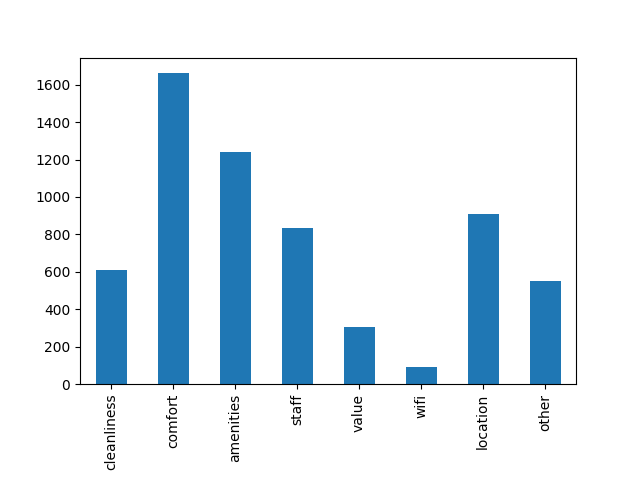
\includegraphics[width=\textwidth]{imgs/acd_y_train_historgram.png}
  		        \caption{ACD task}
  		        \label{acd_y_train_historgram}
		    \end{subfigure}%
		    \begin{subfigure}{.5\textwidth}
 		        \centering
 		        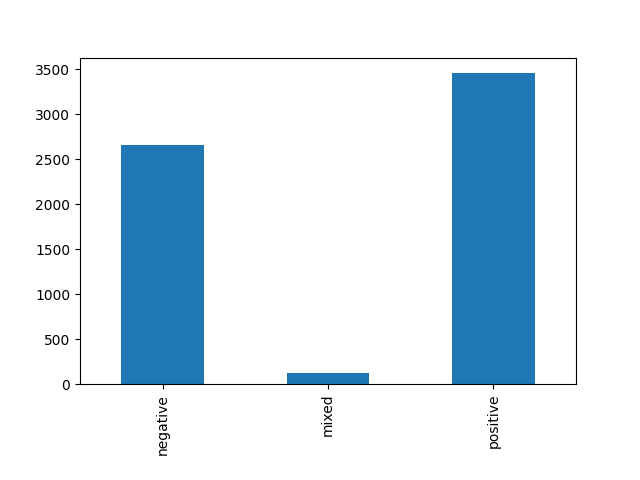
\includegraphics[width=\textwidth]{imgs/acp_y_train_historgram.png}
 		        \caption{ACP task}
 		        \label{acp_y_train_historgram}
		    \end{subfigure}
		    \caption{Number of samples for each class in both training and validation sets}
		    \label{y_train_histograms}
	    \end{figure}
            \begin{figure}
		    \centering
		    \begin{subfigure}{.5\textwidth}
  		        \centering
 		        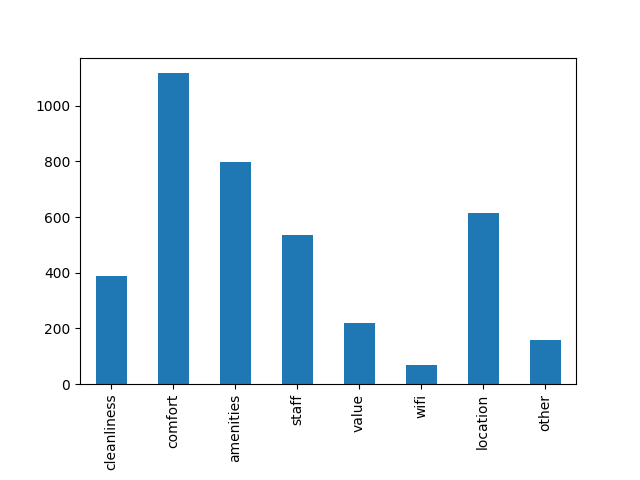
\includegraphics[width=\textwidth]{imgs/acd_y_test_historgram.png}
  		        \caption{ACD task}
  		        \label{acd_y_test_historgram}
		    \end{subfigure}%
		    \begin{subfigure}{.5\textwidth}
 		        \centering
 		        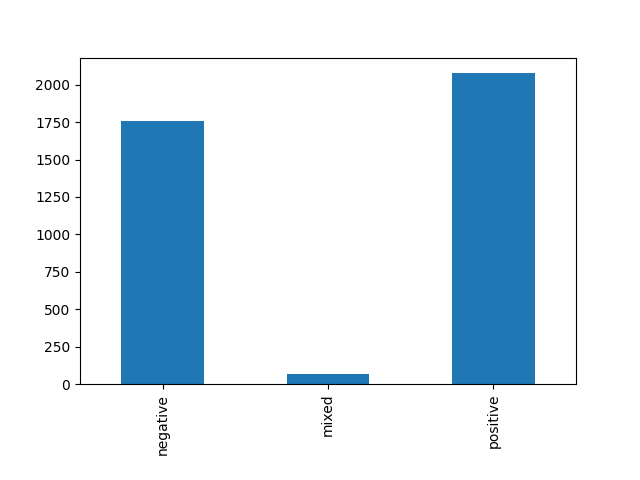
\includegraphics[width=\textwidth]{imgs/acp_y_test_historgram.png}
 		        \caption{ACP task}
 		        \label{acp_y_test_historgram}
		    \end{subfigure}
		    \caption{Number of samples for each class in the testing set}
		    \label{y_test_histograms}
	    \end{figure}
        \subsection{Metrics}\label{subsec:metrics}
        The metrics used for evaluating the models over the tasks used in the Absita evaluation script are micro-precision, micro-recall and f1-score.
        It also gave the macro metrics, but these were not considered.

    \section{Description of the model}\label{sec:s3}
        \begin{figure}
            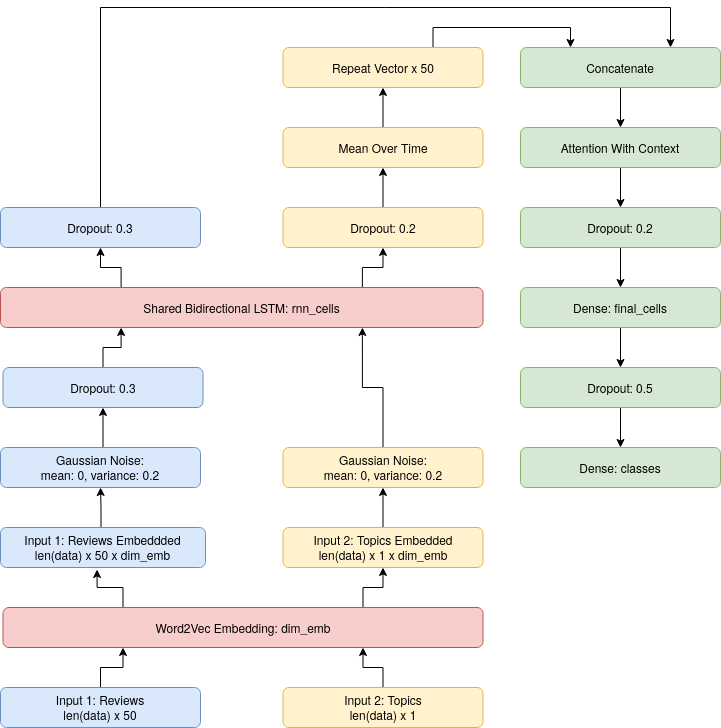
\includegraphics[width=\linewidth]{imgs/model.png}
            \caption{A general view of the model: for the alBERTo version, the reviews are already embedded, and so the input is directly feed into the BiLSTM.
            For for the w2v version, they are embedded in the Embedding Layer.
            The yellow part does not appear for the ACD task, because the task is to find those topics.
            The last dense layer has dimension 3 and softmax activation for ACP task and dimension 8 and sigmoid activation for ACD task.}
            \label{fig:model}
        \end{figure}
        %\subsection{Structure of the models}\label{subsec:structure-of-the-models}%
        The model chosen is the one who outperformed $Semeval2017$, which tasks were very similar to this competition.
        It is a deep-learning model with context-aware attention:
        \begin{itemize}
            \item The inputs are word indices of reviews (and topics for ACP task) to be embedded in the EmbeddingLayer for the Word2Vec version or already embedded for the AlBERTo version
            \item The reviews embeddings are fed into a shared bidirectional LSTM with rnn\_cells neurons.
                For ACP task, it does the same with the topic's embedding using the same weights in order to get meaningful representations
            \item For the ACP task, it concatenates each word representation with the topic representation, repeating the topic representation as many words there are in the review
            \item It uses a context-aware attention mechanism, which tries to understand which part of the reviews contribute more to the sentiment/presence towards the topic
            \item Then it is used a dense layer with final\_cells neurons
            \item Finally there is a dense layer with 8 sigmoid neuron for task ACD or 3 softmax neurons for task ACP
        \end{itemize}
        A more detailed explanation of the model is shown in the image~\ref{fig:model}, with all the dropout layers and gaussian noise layers added to reduce overfitting, and relative parameters.
        Even if we dealt with topics of length of 1 word, there is a MeanOverTime layer after the shared BiLSTM for the ACD task, which computes the mean over time of the words representation which express the topic.
        I implemented this model in $Python$ with the library $Tensorflow$ $2.3.1$, using $Numpy$ and $Pandas$ for array manipulation, $Keras Utilities$ for class weights and callbacks, $Matplotlib$ and $Tensorboard$ for plots and visualizations, $Pycharm$ as preferred editor and $Git$ as version control.
    \section{Preprocessing and embedding information}\label{sec:preprocessing-and-embedding-information}
        The text preprocessing was simple: since the reviews were short and explicit and did not contain emoticons or hashtags, I just removed all the commas, points, quotes and numbers.
        \subsection{w2v}
            Initially I made some experiments using a word embedding whose dimension was 128 (\url{http://www.italianlp.it/resources/italian-word-embeddings/}),
            but this lead to a slow and limited training, that couldn't overtake the accuracy score of 0.55.
            So I moved to a more informative embedding whose size was 300, and, although the poor quality of most of the entries
            (lot of words are typo or sequence of random characters), it gave good results.
            The Italian Word2Vec embeddings (\url{https://arxiv.org/pdf/2001.09332.pdf}) are obtained from a simple 2-level neural network with one-hot vector as input.
            It has been trained with CBOW (continuous bag of words) and negative sampling.
            The dataset was obtained using the information extracted from a
            dump of the Italian Wikipedia (dated 2019.04.01), from the main categories of Italian Google News (WORLD, NATION, BUSINESS,
            TECHNOLOGY, ENTERTAINMENT, SPORTS, SCIENCE, HEALTH), and has a dimension of 2.4 GB .
            Embeddings are given in a txt file, but after the first loading, they are formatted as dictionary and saved in a pickle file to speed up following loading.
            The size of this embedding is 667564 words once removed the non-ascii ones and it could cover the 85\% of the words, but looking better at the words that were indexed as $<unk>$, a lot of them were words with a capital letter.
            So by setting all chars lowercase, without losing much information because no proper name was present in the dataset, and just by removing all \textbf{l'},
            the coverage of word embeddings increased to 91.5\%.
        \subsection{alBERTo}\label{subsec:alberto}
            AlBERTo is the Italian BERT .
            It has the same structure of BERT, the difference is in the learning strategy: BERT is trained with "masked learning" and "next following sentence",
            while alBERTo is trained only with "masked learning".
            Because of this, alBERTo is suitable for sentiment analysis tasks, but not for more complex tasks like QA because it does not have idea of the flow of a dialogue.
            The dataset used to train alBERTo is formed by 200 million of tweets taken from TWITA, which is a big collection of tweets from 2012 since today.
            I used Huggingface Transformers to load the alBERTo model and the tokenizer, then I decided to generate an "alBERTed" version of the dataset,
            in this way I don't need to calculate the embeddings during the training because I have already computed them,
            and this result in a faster training at the cost of spending time and space once and for all to generate and save the embedded dataset.
            The alBERTo tokenizer managed to index all the words.
            The dimension of these embeddings is 768, which is quite larger than the Word2Vec ones.

    \section{Hyperparameters tuning}\label{subsec:hyperparameters-tuning}
            I kept the same dropout values of the original model, and I searched for the best dimensions for the shared bidirectional LSTM rnn\_cells and for the final dense final\_cells layer with a grid search.
            All the models are trained with $Adam$ optimizer, with $clipnorm=0.1$ and $learning\_rate=0.001$.
            I used {64, 128, 256} as domain, and an early stopping callback to speed up the search with $delta=0.01$ and $patience=5$ for alBERTo and $patience=10$ for w2v (because alBERTo learns faster than w2v, as can be seen from the training plots), looking for maximizing the validation recall.
            I obtained the results shown in the tables (ordered by validation recall score), from which I selected the best hidden dimensions for both models and tasks:
            \begin{itemize}
                \item w2v ACD: rnn\_cells 256, final\_cells 256
                \item w2v ACP: rnn\_cells 256, final\_cells 64
                \item alBERTo ACD: rnn\_cells 128, final\_cells 256
                \item alBERTo ACP: rnn\_cells 256, final\_cells 128
            \end{itemize}
                \begin{table}[h!]
                \begin{center}
                \caption{Grid search results for w2v ACD task}
                \label{tab:table6}
                \begin{tabular}{c|c|c|c|c}
                    \textbf{Final cells} & \textbf{BiLSTM cells} & \textbf{Accuracy} & \textbf{Epochs} & \textbf{Validation recall}\\
                    \hline
                        256 & 256 & 0.72397 & 29 & 0.77716\\
                        64  & 256 & 0.72450 & 32 & 0.76312\\
                        128 & 256 & 0.71504 & 19 & 0.76053\\
                        128 & 128 & 0.72766 & 20 & 0.75831\\
                        128 & 64  & 0.71293 & 29 & 0.75721\\
                        64  & 64  & 0.71346 & 29 & 0.75203\\
                        64  & 128 & 0.71767 & 19 & 0.74723\\
                        256 & 128 & 0.70820 & 13 & 0.74501\\
                        256 & 64  & 0.70137 & 10 & 0.73614\\
                \end{tabular}
                \end{center}
            \end{table}
            \begin{table}[h!]
                \begin{center}
                \caption{Grid search results for alBERTo ACD task}
                \label{tab:table5}
                \begin{tabular}{c|c|c|c|c}
                    \textbf{Final cells} & \textbf{BiLSTM cells} & \textbf{Accuracy} & \textbf{Epochs} & \textbf{Validation recall}\\
                    \hline
                        256 & 128 & 0.71504 & 12 & 0.77790\\
                        128 & 256 & 0.72187 & 12 & 0.77605\\
                        64  & 256 & 0.72713 & 15 & 0.77125\\
                        128 & 64  & 0.72397 & 9  & 0.75905\\
                        128 & 128 & 0.71977 & 12 & 0.74982\\
                        64  & 128 & 0.72608 & 11 & 0.74279\\
                        256 & 256 & 0.71609 & 7  & 0.73910\\
                        64  & 64  & 0.73502 & 11 & 0.73651\\
                        256 & 64  & 0.70137 & 9  & 0.73319\\
                \end{tabular}
                \end{center}
            \end{table}
            \begin{table}[h!]
                \begin{center}
                \caption{Grid search results for w2v ACP task}
                \label{tab:table7}
                \begin{tabular}{c|c|c|c|c}
                    \textbf{Final cells} & \textbf{BiLSTM cells} & \textbf{Accuracy} & \textbf{Epochs} & \textbf{Validation recall}\\
                    \hline
                        64  & 256 & 0.91246 & 29 & 0.91096\\
                        64  & 64  & 0.87767 & 22 & 0.87692\\
                        128 & 128 & 0.87580 & 13 & 0.87467\\
                        256 & 128 & 0.87392 & 14 & 0.87168\\
                        128 & 256 & 0.86944 & 13 & 0.86644\\
                        256 & 64  & 0.86756 & 17 & 0.86569\\
                        128 & 64  & 0.85597 & 9  & 0.85297\\
                        64  & 128 & 0.85597 & 6  & 0.84811\\
                        256 & 256 & 0.85036 & 3  & 0.84736\\
                \end{tabular}
                \end{center}
            \end{table}
            \begin{table}[h!]
                \begin{center}
                \caption{Grid search results for alBERTo ACP task}
                \label{tab:table3}
                \begin{tabular}{c|c|c|c|c}
                    \textbf{Final cells} & \textbf{BiLSTM cells} & \textbf{Accuracy} & \textbf{Epochs} & \textbf{Validation recall}\\
                    \hline
                        128 & 256 & 0.91545 & 6  & 0.91470\\
                        256 & 64  & 0.91770 & 10 & 0.91433\\
                        256 & 256 & 0.91358 & 6  & 0.91283\\
                        256 & 128 & 0.91470 & 12 & 0.91171\\
                        64  & 64  & 0.91470 & 6  & 0.91021\\
                        64  & 256 & 0.91246 & 10 & 0.90984\\
                        128 & 128 & 0.90311 & 8  & 0.90086\\
                        128 & 64  & 0.90161 & 5  & 0.89824\\
                        128 & 128 & 0.88178 & 4  & 0.88066\\
                \end{tabular}
                \end{center}
            \end{table}


    \section{Training best models}\label{sec:training-best-models}
            \subsection{ACD}\label{subsec:s2}
            Even if this model was not designed for topic-detection analysis, I wanted to test the potential of the context-aware attention.
            The idea is that the context-aware attention should learn which words refers in a general way to a specific topic.
            So I modified the model in order to be able to do multi-label classification, because more than one topic can be dealt inside the same review.
            The approach is almost the same as for the ACP task, but I removed the part of the model which processed the topics and the output layer has dimension 8 and has a sigmoid activation.

            \subsubsection{Word2Vec}
                The input is a Numpy array with lists of word indices of the reviews.
                The output is a Numpy array with lists of 8 real numbers representing the topic classes ['cleanliness', 'amenities', 'value', 'wifi', 'location', 'staff', 'other'].
                We can see from~\ref{w2v_acd_epoch_loss} that we have an overfitting around the $20^{th}$ epoch, and that the accuracy \ref{w2v_acd_epoch_accuracy} and the recall \ref{w2v_acd_epoch_recall} are quite stable after 10 epochs.
            \begin{figure}
		    \centering
		        \begin{subfigure}{.33\textwidth}
  		            \centering
 		            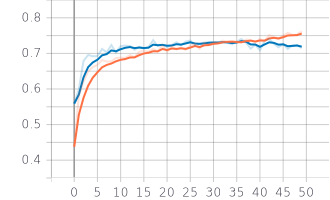
\includegraphics[width=\textwidth]{imgs/plots/w2v_acd_epoch_accuracy.png}
  		            \caption{Accuracy}
  		            \label{w2v_acd_epoch_accuracy}
		        \end{subfigure}%
                \begin{subfigure}{.33\textwidth}
 		            \centering
 		            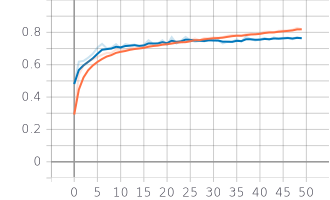
\includegraphics[width=\textwidth]{imgs/plots/w2v_acd_epoch_recall.png}
 		            \caption{Recall}
 		            \label{w2v_acd_epoch_recall}
		        \end{subfigure}
                \begin{subfigure}{.33\textwidth}
 		            \centering
 		            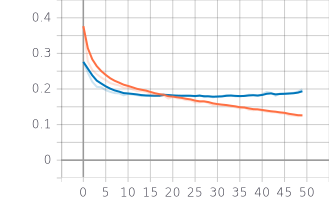
\includegraphics[width=\textwidth]{imgs/plots/w2v_acd_epoch_loss.png}
 		            \caption{Loss}
 		            \label{w2v_acd_epoch_loss}
		        \end{subfigure}
		    \caption{Training history for w2v model in ACD task, x: epochs, y: metric in label.
                    \color{orange} Orange is for train, \color{blue} blue is for validation.\color{black}}
		    \label{w2v_acd_history}
	        \end{figure}

            \subsubsection{AlBERTo}
                The approach is the same as before: I only need to pass the reviews to the model and for each one I will get an array of size 8 with values between [0, 1].
                We see from  \ref{alberto_acd_epoch_accuracy}, \ref{alberto_acd_epoch_recall} and \ref{alberto_acd_epoch_loss} that the training is much faster in this case.
            \begin{figure}
		    \centering
		        \begin{subfigure}{.33\textwidth}
  		            \centering
 		            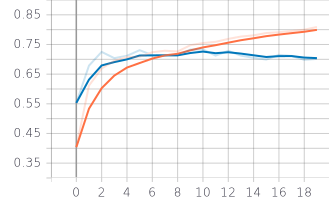
\includegraphics[width=\textwidth]{imgs/plots/alberto_acd_epoch_accuracy.png}
  		            \caption{Accuracy}
  		            \label{alberto_acd_epoch_accuracy}
		        \end{subfigure}%
                \begin{subfigure}{.33\textwidth}
 		            \centering
 		            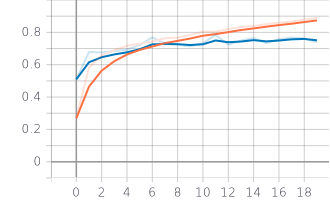
\includegraphics[width=\textwidth]{imgs/plots/alberto_acd_epoch_recall.png}
 		            \caption{Recall}
 		            \label{alberto_acd_epoch_recall}
		        \end{subfigure}
                \begin{subfigure}{.33\textwidth}
 		            \centering
 		            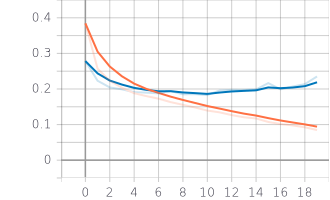
\includegraphics[width=\textwidth]{imgs/plots/alberto_acd_epoch_loss.png}
 		            \caption{Loss}
 		            \label{alberto_acd_epoch_loss}
		        \end{subfigure}
		    \caption{Training history for alBERTo model in ACD task, x: epochs, y: metric in label.
                    \color{orange} Orange is for train, \color{blue} blue is for validation.\color{black}}
		    \label{alberto_acd_history}
	        \end{figure}

        \subsection{ACP}\label{subsec:s1}
            For the ACP task I used class weights, which help dealing with imbalanced datasets by weighting more the misclassified prediction of a class with a limited number of example.
            In this case, the class weights used were 1.26 for $negative$, 1.0 for $positive$ and 8.14 for $mixed$.
            Each review is given multiple times to the model, accordingly to the topics dealt and relative sentiments.
            In this way, the model will learn to distinguish different sentiments towards different topics in the same review.
            \subsubsection{Word2Vec}
            As can we see from \ref{w2v_acp_epoch_accuracy}\ref{w2v_acp_epoch_recall}\ref{w2v_acp_epoch_loss}, the model does not seem to overfit after 50 epochs.
            Anyway, the learning is slow and has high variance, this embedding seems to learn better in the ACD task.
            \begin{figure}
		    \centering
		        \begin{subfigure}{.33\textwidth}
  		            \centering
 		            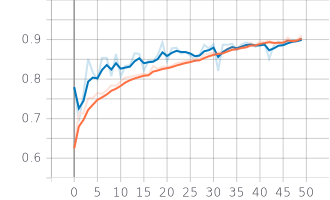
\includegraphics[width=\textwidth]{imgs/plots/w2v_acp_epoch_accuracy.png}
  		            \caption{Accuracy}
  		            \label{w2v_acp_epoch_accuracy}
		        \end{subfigure}%
                \begin{subfigure}{.33\textwidth}
 		            \centering
 		            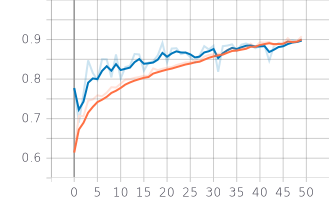
\includegraphics[width=\textwidth]{imgs/plots/w2v_acp_epoch_recall.png}
 		            \caption{Recall}
 		            \label{w2v_acp_epoch_recall}
		        \end{subfigure}
                \begin{subfigure}{.33\textwidth}
 		            \centering
 		            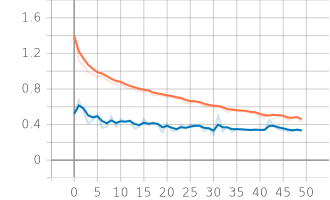
\includegraphics[width=\textwidth]{imgs/plots/w2v_acp_epoch_loss.png}
 		            \caption{Loss}
 		            \label{w2v_acp_epoch_loss}
		        \end{subfigure}
		    \caption{Training history for w2v model in ACP task, x: epochs, y: metric in label.
                    \color{orange} Orange is for train, \color{blue} blue is for validation.\color{black}}
		    \label{w2v_acp_history}
	        \end{figure}
            \subsubsection{AlBERTo}
            As can we see from \ref{alberto_acp_epoch_accuracy}\ref{alberto_acp_epoch_recall}\ref{alberto_acp_epoch_loss}, the training is much faster with respect to the w2v one, and we reach an accuracy of 95\% in just 17 epochs, while with the w2v one we needed 50 epochs to reach an accuracy of 90\%.
            \begin{figure}
		    \centering
		        \begin{subfigure}{.33\textwidth}
  		            \centering
 		            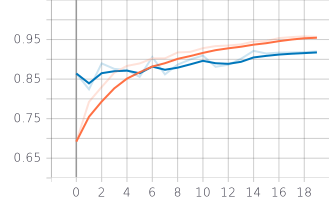
\includegraphics[width=\textwidth]{imgs/plots/alberto_acp_epoch_accuracy.png}
  		            \caption{Accuracy}
  		            \label{alberto_acp_epoch_accuracy}
		        \end{subfigure}%
                \begin{subfigure}{.33\textwidth}
 		            \centering
 		            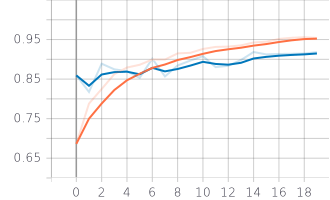
\includegraphics[width=\textwidth]{imgs/plots/alberto_acp_epoch_recall.png}
 		            \caption{Recall}
 		            \label{alberto_acp_epoch_recall}
		        \end{subfigure}
                \begin{subfigure}{.33\textwidth}
 		            \centering
 		            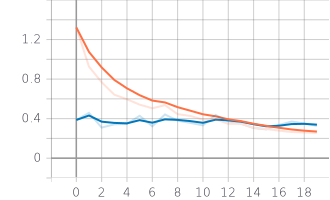
\includegraphics[width=\textwidth]{imgs/plots/alberto_acp_epoch_loss.png}
 		            \caption{Loss}
 		            \label{alberto_acp_epoch_loss}
		        \end{subfigure}
		    \caption{Training history for alBERTo model in ACP task, x: epochs, y: metric in label.
                    \color{orange} Orange is for train, \color{blue} blue is for validation.\color{black}}
		    \label{alberto_acp_history}
	        \end{figure}


    \section{Results}\label{sec:s5}
        As said before, I used the official evaluation\_absita script and the official gold test set (test.csv) to calculate the scores.
        The official evaluation script gives us also the macro measures, but the competition was based on micro measures.
                %ACD RESULTS
                \begin{table}[h!]
                    \begin{center}
                        \caption{Independent results for ACD task}
                        \label{tab:table2}
                        \begin{tabular}{l|c|c|c|r}
                            \textbf{model} & \textbf{Micro-Precision} & \textbf{Micro-Recall} & \textbf{Micro-F1-score}\\
                            \hline
                                \textbf{absita best model} & \textbf{0.8397} & \textbf{0.7837} & \textbf{0.8108}\\
                                W2V & 0.8182 & 0.7468 & 0.7808\\
                                alBERTo & 0.7993 & 0.7814 & 0.7902\\
                        \end{tabular}
                    \end{center}
                \end{table}

                \begin{table}[h!]
                    \begin{center}
                        \caption{Independent results for ACP task}
                        \label{tab:table4}
                        \begin{tabular}{l|c|c|r}
                            \textbf{model} & \textbf{Micro-Precision} & \textbf{Micro-Recall} & \textbf{Micro-F1-score}\\
                            \hline
                                absita best model & 0.8264 & 0.7161 & 0.7673\\
                                W2V & 0.9107 & 0.9006 & 0.9056\\
                                \textbf{alBERTo} & \textbf{0.9388} & \textbf{0.9248} & \textbf{0.9317}\\
                        \end{tabular}
                    \end{center}
                \end{table}
            For the ACD task, we see that both model have results very close to the winner of Absita.
            The w2v model has few higher precision and less than 4 percentage points of recall.
            More accurate results can be obtained with Cross Validation, but it was too costly for my purpose.
            Anyway, in all the experiments I made I always obtained results very similar to the winner of Absita, specially when I moved from a binary class task (my previous approach was: given a review and a topic, understand if that topic was dealt inside the review one at time, repeating review and relative topics like in the ACP task) to a multi-label class.
            I also tried a very simple model with one LSTM with 300 neurons and one dense layer, and model lead to a validation recall of around 74\%, which is not much different from the validation recall of the proposed model, but anyway is less.
            But for the ACP task, we outperform the absita best model with both embeddings by a score of more than 8 percentage points, which is a huge improvement.
            This shows that the the strength of the model is in its idea more than the embeddings, which have a difference of 2/3 percentage points, showing that alBERTo seems to be a better word embedding representation than w2v.

    \section{Conclusion}\label{sec:s6}
        For the ACD task, this model is not so different from the winner of Absita, but this is not surprising because this model was initially designed for the ACP task.
        model is very good at understanding the sentiment expressed toward a certain topic, and it can also understand
        if the sentiment is mixed, and if different topics have different sentiments in the same review.
        The role of the context attention is crucial in the topic based sentiment analysis, because it can understand well which words express a certain sentiment towards a certain topic.
        Moreover, alBERTo embeddings are better than W2V one, in both test results and learning speed (alBERTo model overfits faster than the w2v one, but with a higher score).
        This could depend on the bigger embedding dimension (768 vs 300), the model used to obtain them
        (multiple transformers vs simple neural network) and the learning strategy (CBOW vs masked learning).

\end{document}